\documentclass[titlepage, 12pt, a4paper]{article}
\usepackage[utf8]{inputenc}
\usepackage{hyperref}
\usepackage{csquotes}
\usepackage{listings}
\usepackage{float}
\usepackage{graphicx}
\usepackage{mathptmx}
\usepackage{comment}
\usepackage[
backend=biber,
style=alphabetic,
sorting=ynt]{biblatex}
\usepackage{anysize}
\usepackage[spanish]{babel}

%Paragraph format
\setlength{\parindent}{2em}
\setlength{\parskip}{1em}

% color in page
\usepackage{afterpage}
\usepackage{xcolor}
\usepackage{pagecolor}
\definecolor{u-blue}{RGB}{32,2,116}

% Margin sizes for page
\marginsize{3cm}{3cm}{2.5cm}{2.5cm}
 
\usepackage[nonumberlist,acronymlists={gloss}]{glossaries}
\makeglossaries

\newglossaryentry{latex}
{
	name=latex,
	description={A markup language}
}


\addbibresource{bibliography.bib}
\title{\color{white}Análisis y automatización de doble factor de autenticación en sistemas GNU/Linux}
\author{\color{white}Roselló Morell, Sergio\\
\texttt{\color{white}sergio.rosello@live.u-tad.com}}

\begin{document}

\newpagecolor{u-blue}
\afterpage{\restorepagecolor}
\maketitle
\section*{Agradecimientos}
Debo agradecer a Eduardo Ariols, mi tutor del trabajo todo el apoyo y consejos dados. Estoy seguro de que sin su ayuda, este trabajo no hubiese llegado a su nivel actual. Durante el proceso de elección del trabajo, me ayudó a darme cuenta de lo que quería hacer exactamente y desde ese momento, no ha parado de inspirarme con distintas formas de ver las cosas. De eso, le estoy muy agradecido.\par También quiero agradecer a la universidad el buen trabajo a la hora de escoger al personal docente de mi grado, puesto que en todo momento han demostrado más que profesionalidad y compañerismo hacia mi y mis compañeros de carrera.
\clearpage
\section*{Resumen}
Este documento explica al lector la experiencia que he tenido durante el periodo de realización del trabajo de final de grado. Este trabajo trata sobre la autenticación de un usuario a un sistema \Gls{GNU/Linux}, en concreto, mediante una llave \Gls{USB}.\par Durante la fase de investigación de las tecnologías existentes, encontré algunas que ofrecían usa solución elegante, mediante \Gls{dbus} pero acabando la fase de investigación encontré un proyecto llamado \Gls{PAM} que redefinió la forma en la que planteaba el trabajo. Ésta es la forma por defecto de autenticar a los usuarios que tienen la mayoría de sistemas \Gls{GNU/Linux}.\par Este trabajo, al principio con enfoque mucho más práctico ha acabado teniendo un enfoque investigativo puesto que para implementar el módulo de autenticación, he tenido que construir una base fuerte sobre la que sentirme cómodo. Esta base es la que he tenido que esforzarme a entender puesto a que sin ella, el trabajo realizado, aunque funcionalmente completo, no me hubiese sido ni la mitad de estimulante e interesante.
\begin{abstract}
This document reports my experience as I work on creating a USB-centric authentication method for \Gls{GNU/Linux}. During the research phase, I came across several elegant implementations, all of them worked with \Gls{dbus}. During the final stages of this period, I discovered \Gls{PAM} which changed my whole perspective on this project. Most of \Gls{GNU/Linux} systems use this module to enable authentication for their users.\par At the start of this project I would've expected to code a lot more, but now I realise that without a solid foundation, I may have been able to do what I had proposed, but I would not have the understanding on how the \Gls{PAM} fits into the whole equation and the many benefits it provides. This, I think is the point of this work.
\end{abstract}
\tableofcontents
\clearpage
\listoffigures
\clearpage
\printglossary[title={Abreviaciones y tecnicismos}]
\clearpage
\section{Estado del arte}
\subsection{Evolución de las tecnologías}
Los ordenadores forman una gran parte de nuestra sociedad desde que fueron inventados. El primer ordenador que se creó fue el Mark I, en 1944. Este ordenador estaba hecho mayoritariamente para realizar cálculos, pesaba cinco toneladas y se sobrecalentaba.
Desde Mark I, como podemos observar en la imagen \ref{fig:moore}, los ordenadores han ido duplicando el número de transistores en circuitos integrados cada dos años \cite{moore}. Hasta ahora, y seguramente unos años más en adelante, podamos ver que se sigue cumpliendo la ley de Moore.
\begin{figure}[H]
    \centering
    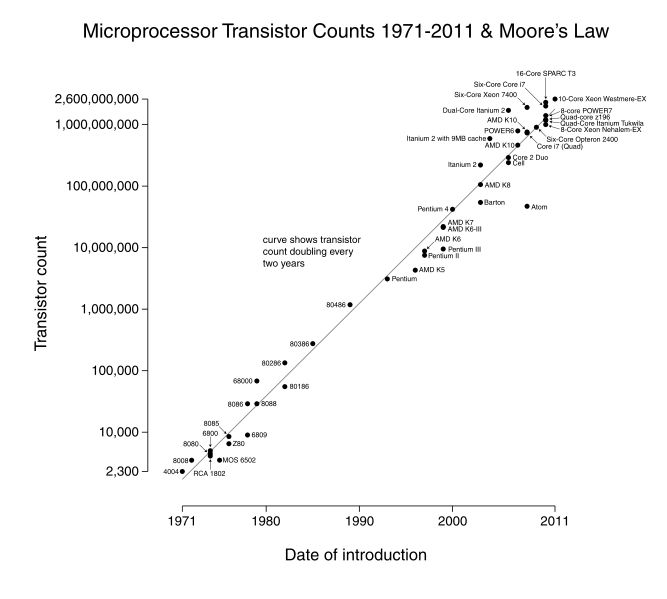
\includegraphics[width=0.5\textwidth]{Media/moore.jpg}
    \caption{Ley de Moore}
    \label{fig:moore}
\end{figure}
Durante el periodo de evolución de la informática, se pueden diferenciar cinco generaciones:
\begin{itemize}
	\item{\textbf{Primera generación: }}Estos ordenadores no se parecían en nada a los ordenadores modernos, eran extremadamente grandes y poco sofisticados. Eran estructuras tan grandes como una habitación entera y usaban válvulas termodinámicas como switches y amplificadores. Las válvulas termodinámicas generaban mucho calor así que a pesar de contar con unidades de refrigeración enormes, se sobrecalentaban muy frecuentemente.\par Para interaccionar con estos ordenadores, los programadores usaban un lenguaje conocido como "Lenguaje de máquina" que era directamente interpretable por el circuito.\par Esta generación tuvo lugar entre los años 1940 y 1956
	\item{\textbf{Segunda generación: }}Estos ordenadores se distinguen de la primera generación porque consiguen sustituir las válvulas termodinámicas por el  transistor. El cambio de válvulas a transistor implica más velocidad de cálculo y menos energía residual el forma de calor. Otra de las ventajas de los transistores es que, al ser más pequeños, reducen el tamaño del ordenador y lo hacen más económico.\par En esta generación, también se consiguió almacenar información en discos, siendo esta la primera forma de almacenamiento de información persistente.\par Esta generación tuvo lugar entre los años 1956 y 1963.
	\item{\textbf{Tercera generación: }}Se implementaron por primera vez los circuitos integrados, que contenían muchos transistores en chips semiconductores. Las ventajas de esta aportación fueron velocidad de cálculo, que aumentó mucho, el tamaño se redujo considerablemente y se continuaron abaratando los precios. En vez de "Lenguaje máquina", ahora los programadores usan monitores y teclados para comunicarse con el ordenador. Hasta esta generación, los ordenadores no estaban destinados para un uso personal. Solo las grandes empresas podían permitirse tener un ordenador.\par Esta generación tuvo lugar entre los años 1964 y 1971.
	\item{\textbf{Cuarta generación: }}Es la generación con más impacto en la sociedad. La tecnología avanzó hasta tal punto que los fabricantes podían poner miles de transistores en un único circuito integrado. EN esta época se puso a la venta el Intel 4004, el primer microprocesador en venderse de forma masiva. Este desarrollo inició la industria de los ordenadores personales.\par A mediados de los 70, salieron al mercado ordenadores como el Altair 8800 que venían a piezas y su usuario tenía que construir para usar. A finales de los 70, inicios de los 80, salieron al mercado ordenadores construidos de fábrica, como el Comodore pet, Apple II y el primer ordenador IBM. Al inicio de los 90, los ordenadores personales y la capacidad de crear una red de comunicación entre ellos dio paso a la creación de Internet. Se mejoró también la capacidad de almacenamiento de los discos además de la velocidad en general. Aparecieron lor primeros ordenadores portátiles, que presentaban una \Gls{GUI} para facilitar la interacción entre el usuario y la máquina.\par Los usuarios de los ordenadores ya no tenían que ser gente técnica ni debía realizar un curso de formación para saber usarlos. Esto avivó la tasa de adopción de esta tecnología enormemente.\par Esta generación tuvo lugar entre los años 1971 y 2010.
	\item{\textbf{Quinta generación: }}Actualmente nos encontramos en esta generación. Algunos dicen que la adopción de los ordenadores cuánticos es el próximo gran paso, pero desde mi punto de vista, aún queda bastante para que eso ocurra.\par Creo que la quinta generación se caracterizará por el cambio de mentalidad de los usuarios de ordenadores. Hoy en día, tener la información guardada en un ordenador ya no es un privilegio, ni una ventaja competitiva. La verdadera ventaja es la disponibilidad de la información en cualquier ordenador al que te conectes, proporcionando al usuario una forma de acceso a información revolucionaria. Nunca antes ha sido posible acceder desde cualquier sitio a la información de un usuario.\\Esta generación empezó en 2010.
\end{itemize}
Ha sido a partir de la cuarta generación cuando los desarrolladores de aplicaciones han tenido que preocuparse de verificar que las credenciales que usan sus usuarios son correctas. Originariamente, \Gls{GNU/Linux} no tenía un método de autenticación definido. Esto significa que cada desarrollador gestionaba la autenticación del usuario de una forma distinta. Para los desarrolladores, esto significaba más tiempo perdido implementando medidas de seguridad que no guardan relación con el contenido de sus aplicaciones y para los administradores de sistemas significaba que tenían que mantener diversos métodos de autenticación (uno para cada aplicación) actualizados para seguir cumpliendo los estándares de seguridad deseados. \par
Existían dos mentalidades para realizar la autenticación del usuario, la primera consiste en buscar los nombres y hashes de los usuarios en los archivos /etc/passwd y /etc/shadow y compararlo con lo que había introducido el usuario. La segunda mentalidad directamente gestionaban la autenticación de la forma que querían. \par
Como era de esperar, al no haber ni estándar ni protocolo, urgía una solución rápido. En 1995, \Gls{Sun} propuso un mecanismo llamado \Gls{PAM}. Este mecanismo proporcionaba a los desarrolladores de aplicaciones una \Gls{API} que se ocupaba de manejar la lógica de autenticación y beneficiaba al administrador de sistemas porque unificaba el control de autenticación en un solo sitio, que además, permitía implementar distintos esquemas de autenticación.
\subsection{Consecuencias de la evolución}
El rápido desarrollo de esta tecnología, como era de esperar cuando las cosas se hacen rápido y a contra reloj, introdujo un factor de error en la ecuación. Desde los inicios, ya sea por fallo humano o casualidad, se habla de un fenómeno llamado \textit{\Gls{bug}}. Este término forma parte de la jerga informática desde 1947, año en que, durante el ensamblaje del ordenador \textit{Harvard Mark II}, tras el incorrecto funcionamiento del ordenador, los ingenieros revisaron las conexiones del ordenador y se encontraron con un insecto que adherido a dos cables, provocaba el fallo en el sistema. Desde entonces, se llama \textit{\Gls{bug}} al fallo en un programa, ya sea lógico o sintáctico.\par Debido a la rápida adopción de los ordenadores por la población se continuó produciendo software con \textit{\Gls{bug}s}. Un estudio realizado por el \textit{\Gls{NIST}} concluyó en que los fallos en el software le cuestan a la economía estadounidense 59.5 billones de dólares anuales.\cite{NIST}\par A medida que más usuarios usan programas, se van encontrando nuevos fallos, que dependiendo de la escala de gravedad podrían ser críticos, tanto para las empresas como para sus usuarios ya que si un usuario con malas intenciones encuentra un fallo de seguridad en la aplicación, dependiendo de su gravedad, podría, en teoría obtener información sensible de otros usuarios además de información interna de la compañía que ha hecho el software.\par Para combatir este problema, algunas empresas han decidido recompensar a los usuarios que encuentran estos fallos. Al ofrecer una recompensa económica, la empresa incita al usuario a describir el fallo para que se pueda arreglar. Este tipo de programa se llama \Gls{bbp}. Existen varias páginas que se dedican a gestionar las ofertas de las empresas y los hallazgos de los usuarios para que ambos salgan ganando.\par Hoy en día, tenemos todos nuestros datos \textit{on-line}. Esto nos ofrece grandes ventajas como el acceso inmediato a nuestra información personal pero corremos un gran riesgo al confiar en las empresas que hacen que esto sea posible porque no existen programas sin  \textit{\Gls{bug}s}.
\subsection{Necesidad de seguridad}
A medida que ha ido evolucionando la tecnología, medidas de seguridad previamente válidas, han ido quedando deprecadas debido a fallos que se han encontrado en los protocolos o nuevas versiones de estas mismas. El campo de la seguridad en la informática ha ido evolucionando como si se tratara del juego del ratón y el gato en el que los desarrolladores arreglan e inventan nuevas formas de proteger la información de los usuarios y los hackers vulneran esas implementaciones.\par Ahora mismo, los usuarios son los que más tienen que perder. Tenemos todos nuestros datos almacenados en servidores de grandes empresas como Google o Facebook y en el caso de que se filtre nuestra información al mundo, tanto fotos personales como documentos sensibles se verían expuestos a todos los usuarios de Internet.\par Para evitar esto, estas empresas implementan métodos de seguridad cada vez más avanzados como el doble factor de autenticación para iniciar sesión en la cuenta.\par Las medidas de seguridad que proporcionan las empresas como Google o Facebook son bastante buenas pero no son suficientes. Tampoco podemos pedir a estas empresas que implementen todo tipo de sistemas de autenticación de usuarios, ya que al final, tienen que hacer el proceso fácil y sencillo para que le gente quiera y sepa usarlo.\par Podemos aumentar la seguridad de nuestro sistema configurando nosotros mismos las distintas formas de autenticarnos en nuestros sistemas. Una de las formas en las que podemos aumentar la seguridad de nuestro sistema es mediante el \Gls{dfa}. Algunos ejemplos de esta implementación son:
\begin{itemize}
	\item Contraseña + Llave USB
	\item Contraseña + App generadora de códigos (Google Authenticator)
	\item App generadora de códigos + Sensor de huella dactilar
	\item Contraseña + Sensor de retina
\end{itemize}
A cuanto más valor, ya sea económico o emocional, más medidas de seguridad serán implementadas en proteger dicha información.\par En definitiva, es muy complicado tener un entorno seguro en el que poder confiar porque muchas de los vectores de ataque no dependen del usuario final, sino de terceros (Tantos como distintos servicios use el usuario). Es importante tener un buen nivel de seguridad en todos los dispositivos, pero este no debe interponerse entre las tareas que un usuario tiene que hacer en su ordenador ya que de lo contrario, sería un inconveniente, no una ventaja. Cada usuario debe establecer el grado de seguridad de sus cuentas, tanto en Internet como de sistema.\par Creo que existe una relación fuerte entre las medidas de seguridad que implementan los usuarios y el valor de la información que esa información tiene para ellos. Para la mayoría de usuarios, una contraseña, aunque menos segura que un \Gls{dfa} será más conveniente porque la naturaleza de la información que tiene que proteger no es tan importante.
\section{Introducción}
\subsection{Motivación}
Como todo alumno de primero de carrera, inicié el curso con ganas y Windows.\par En primero ya me di cuenta de que no era el mejor sistema operativo para desarrollar. Cada vez que usaba una máquina virtual para hacer cualquier práctica, me planteaba cambiarme a \Gls{Ubuntu} y dejar atrás Windows.\par Al empezar segundo de carrera, decidí hacer una partición para \Gls{Ubuntu}. De esta forma, no tenía que iniciar una máquina virtual en Windows para trabajar. Durante dos años estuve usando este sistema pero no estaba contento porque no satisfacía mi curiosidad. Sabía que no era mi sistema operativo.\par Durante el verano del tercer año en la carrera decidí que quería cambiar a \Gls{Arch linux} pero vi varios comentarios en foros que sería mejor pasar antes por \Gls{Manjaro} para acostumbrarme al ecosistema de \Gls{Arch linux} y coger soltura y confianza interaccionando con mi ordenador desde la consola.\par Entrando en el segundo cuatrimestre de cuarto (Quinto año en la carrera) me sentía lo suficientemente cómodo como para instalar \Gls{Arch linux} en mi sistema.\par Todo el proceso de aprendizaje que he pasado durante estos años me ha servido para aprender y valorar el sistema operativo.\par Esta es la razón por la que supe desde el primer momento en que nos dijeron que fuésemos pensando sobre que queríamos hacer el trabajo de fin de grado que quería hacerlo sobre \Gls{GNU/Linux}.\par Trás toda esta experiencia, he querido ampliar mis conocimientos en \Gls{GNU/Linux}. Durante la reunión con mi tutor, vimos algunas opciones de investigación y finalmente, al estar interesados en la seguridad de las aplicaciones y sistemas, decidimos que era buena idea tirar por esa rama.\par Durante el transcurso de la carrera, ya sea por requisito de los profesores o por mis proyectos personales, he sido un gran usuario del software de control de versiones, \Gls{Git}. Lo he usado desde prácticas en las que era necesario hasta para este mismo documento. Desde que empecé a usarlo, vi que no se trataba simplemente de una herramienta para gestionar mis proyectos, sino de un estilo de vida, una forma de enseñar y compartir los proyectos en los que estás involucrado.\par La mayor parte de los programas que uso en mi sistema operativo se desarrollan de forma abierta en los que puedes ver el progreso y interaccionar con los desarrolladores, incluso ayudarles a detectar errores o solicitar un \textit{push request} para arreglar algún fallo.\par Por este motivo, solicitaré un \textit{push request} al usuario del cual me he basado para hacer mi trabajo de fin de grado.
\subsection{Descripción del proyecto}
Durante la búsqueda de documentación sobre \Gls{PAM} y como debería implementar el módulo que se encarga de autenticar al usuario mediante
un dispositivo \Gls{USB} encontré en \Gls{GitHub} un proyecto que hacía exactamente lo que tenía pensado implementar yo. Al ya existir esto, vi que no tenía sentido reinventar la rueda, así que decidí crear un \Gls{script} en \Gls{bash} que facilitase al usuario no técnico la configuración del módulo \Gls{USB} para el \Gls{PAM}.\par
El \Gls{script} que he creado ayuda al usuario a seleccionar el \Gls{USB} que quiera usar, le explica las diferencias entre las distintas formas que hay de configurar el Módulo y le deja decidir donde quiere introducir la línea de configuración ya que al ejecutar las órdenes de forma secuencial, dependiendo de la posición en la que se coloque la línea, el módulo hará una cosa o otra. \par
Previo a mi \Gls{script}, para configurar el módulo \Gls{USB}, el usuario debía leer la documentación oficial de PAM para averiguar que archivo es el que debe configurar y como lo debe hacer. Lo que consigo con mi \Gls{script} es reducir la curva de aprendizaje necesaria para configurar un método de autenticación más seguro que el de la contraseña por defecto. Esto hará que más usuarios tengan acceso a mejor autenticación en sus ordenadores sin que pierdan conveniencia y comodidad.
\subsection{Competencias adquiridas}
Durante el desarrollo del proyecto, he desarrollado tanto aptitudes como actitudes. A continuación describiré tanto las situaciones en las que he demostrado una actitud como las aptitudes que he desarrollado y reforzado.
\subsubsection{Aptitudes adquiridas o reforzadas}
\begin{itemize}
	\item{\textbf{\Gls{bash}}}\par Decidí usar este lenguaje de progrmamación para hacer el script porque sabía que no me iba a encontrar con complicaciones a la hora de asegurar que funcione en cualquier equipo ya que todos los programas usados en el script vienen instalados de forma predeterminada en la gran mayoría de sistemas.
	\item{\textbf{\Gls{C}}}\par El \Gls{PAM} está escrito en \Gls{C} y he tenido que leer y entender como funciona el submódulo USB para ver como se comunican ambos módulos.
	\item{\textbf{\Gls{Python}}}\par En la primera implementación que hice, usé este lenguaje de programación para bloquear la pantalla del ordenador mediante \Gls{dbus}.
	\item{\textbf{\Gls{Linux}}}\par Durante el transcurso del proyecto he estado investigando el funcionamiento de \Gls{Linux} aunque más detalladamente en los mecanismos de autenticación de usuarios que tiene.
\end{itemize}
\subsubsection{Actitudes adquiridas o reforzadas}
\begin{itemize}
	\item{\textbf{Resolutivo}}\par Durante la primera iteración de investigación/implementación, encontré una forma de desbloquear el equipo mediante \Gls{dbus}. Esta forma, aunque funcional, no es elegante. Es más parecido a un ``hack" que a una solución elegante y segura. Si no hubiese ``dado un paso atrás", no hubiese continuado investigando/implementando otras soluciones. \par Cuando encontré PAM\_USB, me obcequé en hacer que funcionase, ya que si no funcionaba, no podía avanzar en el trabajo. De nuevo, tuve que dar un paso atrás para buscar otras implementaciones para el módulo \Gls{PAM} con \Gls{USB}.
	\item{\textbf{Persistencia}}\par Guarda una relación directa con la forma en la que he enfocado el trabajo.
	\item{\textbf{Adaptabilidad}}\par Durante toda mi vida de estudiante, mi forma de retener la información y por consiguiente aprender, ha sido escuchando al profesor. Leer los apuntes a mi me sirve como refuerzo a la explicación del profesor. Durante este proyecto, no he seguido esa misma dinámica, ya que no he tenido un profesor a quien escuchar, he tenido que investigar y formarme a base de la lectura de las páginas de documentación y los comentarios informativos en el código.
\end{itemize}
\subsection{Estructura del documento}
Ahora mismo no se que poner ;) ***
\section{Objetivos}
Desde el inicio, el principal objetivo de este trabajo ha sido expandir mi conocimiento sobre \Gls{GNU/Linux}. Además de ser un sistema operativo versátil y fehaciente, es una prueba viviente de que se puede hacer código libre en comunidad y de calidad. Al hablar con mi tutor mi idea sobre el trabajo, concluimos en que tendríamos que hilar más fino, entonces, me sugirió centrarnos en la seguridad. \par
Una vez reducido el ámbito de investigación, debía encontrar un proyecto que me interesase. Tuve la suerte de que mi tutor me parara el enlace de un vídeo en el que se describía como se generaba una puerta trasera en el sistema, mediante herramientas poco monitorizadas por los administradores de sistema debido a la cantidad de tráfico que generan. Este proyecto me interesó y decidí centrar mi investigación en el análisis y la automatización de doble factor de autenticación en sistemas \Gls{GNU/Linux}. \par 
Mi objetivo inicial en este trabajo era crear un sistema que permitiese al usuario bloquear y desbloquear el ordenador con un \Gls{USB}. Cuando empecé a investigar como podía hacer eso, me centré en \Gls{dbus}. Tras el primer ciclo de investigación/implementación conseguí bloquear el sistema al enviar un comando mediante \Gls{dbus} al programa que se encarga de bloquear el sistema pero debido a varios factores que se explicarán más adelante, no era una solución buena. \par 
Buscando alternativas, encontré \Gls{PAM}. Cuando averigüé que era la forma por defecto de autenticación de usuarios en la mayoría de sistemas \Gls{GNU/Linux} y vi que ya estaba diseñada para permitir múltiples factores de autenticación, supe que usar PAM era el camino que debía seguir. \par
Para avanzar, ahora debía entender como funcionaba PAM y como crear un módulo de autenticación por \Gls{USB} que lo implementara. Este fue mi siguiente objetivo. \par
Al ver que ya existía un módulo que hacía justamente eso, me centré en facilitar la adopción de este módulo a los usuarios, de forma que más gente no técnica pueda acceder a mejor autenticación.
\section{Métodos de trabajo}
Al empezar el trabajo tenía claro que quería seguir una metodología de desarrollo ágil, ya que a mi parecer, es la evolución del desarrollo en cascada y aporta muchas ventajas al flujo de trabajo.
\begin{figure}[H]
    \centering
    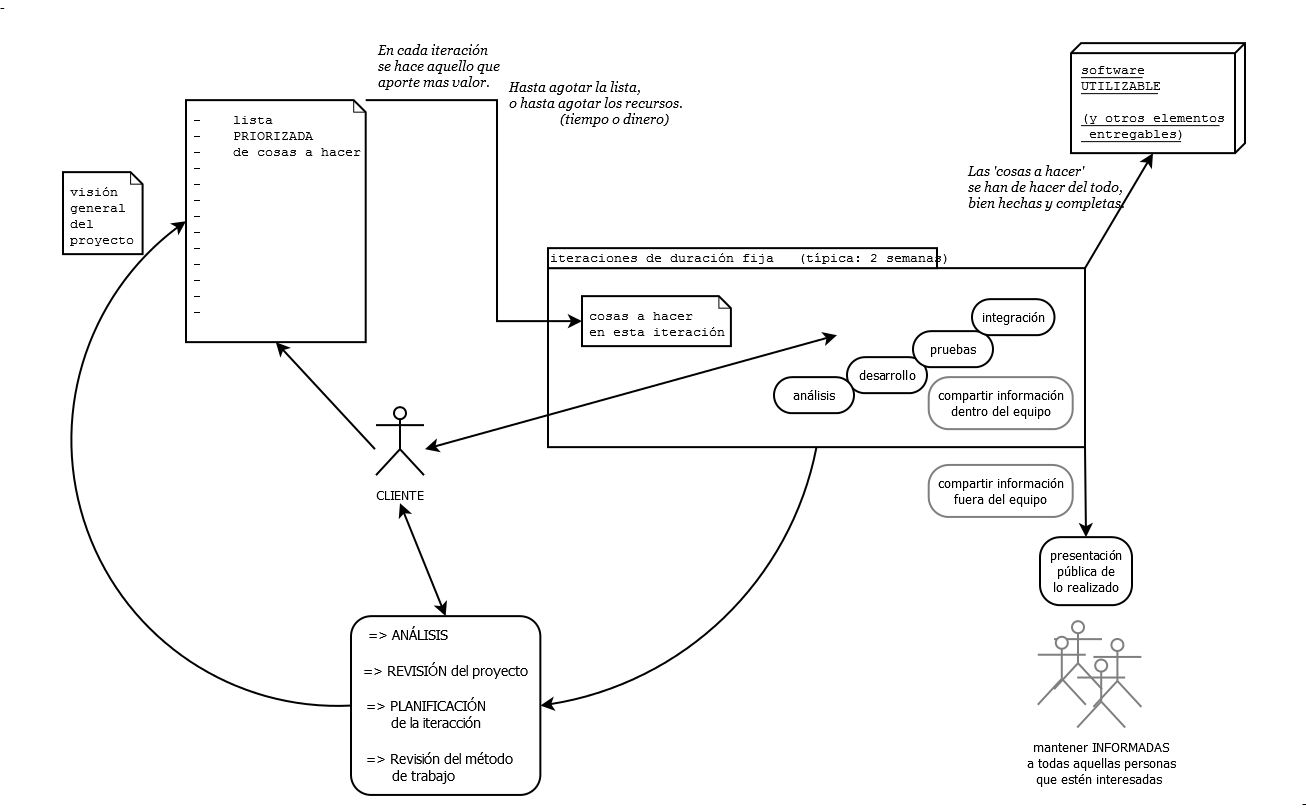
\includegraphics[width=1\textwidth]{Media/agile.png}
    \caption{Diagrama explicativo de una Metodología ágil}
    \label{fig:agileMethodology}
\end{figure}
Esta metodología se basa en una serie de ideas que quedan bien plasmadas en su manifiesto. Esto es, aunque valoramos los elementos de la derecha, valoramos más los de la izquierda.\cite{agile} 
\begin{itemize}
	\item{\textbf{Individuos e interacciones} sobre procesos y herramientas}
	\item{\textbf{Software funcionando} sobre documentación extensiva}
	\item{\textbf{Colaboración con el cliente} sobre negociación contractual}
	\item{\textbf{Respuesta ante el cambio} sobre seguir un plan}
\end{itemize}\par
Las ventajas de este estilo de desarrollo frente a estilos más conservadores como el de cascada son, entre otras que el cliente trabaja con el equipo de desarrollo constantemente para adaptar el producto a las características deseadas, el flujo de trabajo se basa en la repetición de actividades como análisis de requisitos, diseño, implementación, testeo y producción de forma iterativa hasta conseguir un producto acabado.\par
Diría que he seguido bastante de cerca el estilo de desarrollo propuesto por esta metodología. Durante el periodo de desarrollo del trabajo, he mantenido una relación cercana con mi tutor, manteniéndole siempre al día sobre los progresos del proyecto, cada semana aproximadamente nos reuníamos para ver el estado del proyecto, en la que le describía los progresos prácticos conseguidos. Cuando decidimos que \Gls{dbus} no era una buena solución, supe responder al cambio y adaptar el proyecto a nuevas y mejores soluciones. \par
A medida que avanzaba el proyecto, el área de investigación se volvía más pequeña y enfocada. Durante las primeras semanas, me centré en investigar el transcurso de los métodos de autenticación. Una vez analizadas las distintas formas de autenticación, profundicé en \Gls{dbus}, implementé un programa que enviaba un mensaje mediante este bus al programa encargado de bloquear y desbloquear el sistema y conseguí bloquear el sistema. Esto me servía como prueba de concepto pues si había logrado bloquear, solo faltaba añadir una capa de abstracción más que enviase el comando de bloqueo si las acciones del usuario cumplían con el comportamiento esperado. \par
Durante el periodo de investigación de dispositivos con los que podía realizar un \Gls{dfa} llegué a la conclusión de que en realidad cualquier dispositivo hardware es válido. Cuando alguien piensa en \textit{\Gls{dfa}}, lo más común es pensar en las aplicaciones como Google Authenticator. Lo siguiente que viene a la mente es usar una llave \Gls{USB} como segundo factor de autenticación, pero la realidad es que se pueden usar todo tipo de dispositivos, algunos ejemplos son: auriculares (comprobando que se complete un patrón como por ejemplo insertar y extraer el jack de audio dos veces seguidas), una tarjeta de red \textit{\Gls{wifi}} (comprobando  el \textit{\Gls{finterprint}} de los dispositivos que emiten una señal \textit{\Gls{wifi}} con una lista de \textit{\Gls{fingerprint}s} aceptados) o cualquier módulo \Gls{bluetooth} (comprobando el \textit{\Gls{fingerprint}} contra una lista de \textit{\Gls{fingerprint}s} aceptados). Solamente es necesario que el sistema operativo lo reconozca. \par
Finalmente, tras investigar las ventajas e inconvenientes de varios dispositivos hardware, me decanté por el \Gls{USB} como segundo método de autenticación. Aunque otros dispositivos como auriculares pasan desapercibidos, el sistema de verificación no puede interactuar con ellos y aunque no sea una necesidad, el hecho de poder interactuar con el \Gls{USB}, me proporciona más formas de verificar al usuario.
\section{Investigación y resultados}
En esta sección, describiré las distintas tecnologías de autenticación existentes, los problemas actuales de esas tecnologías, defenderé la necesidad de una seguridad más agresiva, tanto para los usuarios normales como para las grandes empresas y desglosaré las distintas formas de conseguir esta seguridad actualmente.
\subsection{Tecnologías y protocolos}
La forma en la que se autentica la identidad de los usuarios de sistemas ha ido evolucionando desde que se vio que era necesaria.
\subsubsection{Inicios de la gestión de permisos}
Cada objeto tiene asociada una tabla de 9 bits, los tres primeros indican los privilegios de lectura, escritura y ejecución del usuario que posee el objeto. Los tres siguientes son para la lectura, escritura y ejecución de los usuarios pertenecientes al grupo que posee el objeto y los tres últimos son de lectura, escritura y ejecución de los usuarios que no pertenecen a ninguno de las dos primeras categorías. Esta categoría se llama \textit{others}. Además de estos 9 bits, también pueden incluir el \Gls{SetUid}, \Gls{SetGid} y el \Gls{StickyBit}. A pesar de ser un sistema muy simple de gestionar privilegios, cumple la mayoría de escenarios posibles en sistemas UNIX e incluso a día de hoy, se sigue usando en todos los sistemas \Gls{GNU/Linux} ya que proporciona una forma sencilla y eficiente de visualizar los privilegios de los objetos y modificarlos. Esta forma de gestionar los privilegios de los objetos se puede denominar \Gls{ACL}.
\begin{figure}[H]
    \centering
    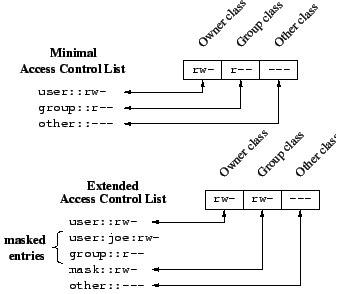
\includegraphics[width=0.5\textwidth]{Media/ACL.jpg}
    \caption{\Gls{ACL}}
    \label{fig:ACL}
\end{figure}
\subsubsection{\Gls{RBAC}}
Este esquema de seguridad está diseñado para organizaciones o sistemas en los que van a interactuar distintos usuarios con una gran cantidad de datos. El sistema defiende que, en lugar de tener una tabla por cada objeto, definiendo la forma que tienen los usuarios de interactuar con él, se deberían establecer una serie de transacciones, que dependiendo del rol serán distintas. Estas transacciones, una vez definidas cambian poco porque un usuario específico va a usar unos documentos específicos, dependiendo de la responsabilidad que tenga en la organización. En la imagen \ref{fig:RBAC} se puede ver claramente como dependiendo del rol vas a poder acceder a ciertos objetos.
\begin{figure}[H]
    \centering
    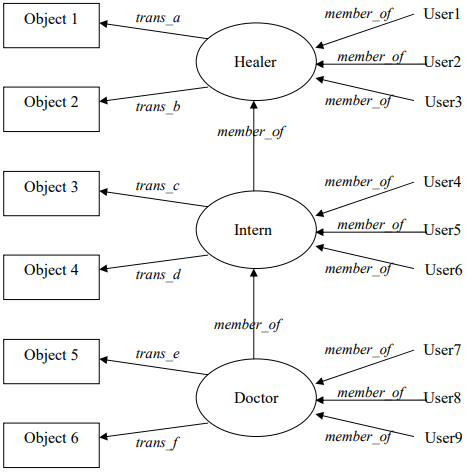
\includegraphics[width=0.5\textwidth]{Media/RBAC.PNG}
    \caption{\Gls{RBAC}}
    \label{fig:RBAC}
\end{figure}
Dos de las ventajas de este sistema son que cumplir el principio de de menor privilegio es relativamente sencillo, ya que se puede conseguir no proporcionándole  al usuario más transacciones de las que debe tener. Otra de las ventajas, innata, de \Gls{RBAC} es la separación de deberes. Esto es: En el caso de tener que realizar un transferencia bancaria, nunca se debería de poder proporcionar al mismo individuo el control de todo el flujo, ya que se le está dando la oportunidad de cometer algún tipo de irregularidad. Con RBAC puedes asignar dos transacciones, una que permita a un usuario solicitar una transferencia y otra que permita a un usuario validar la transferencia.
\subsubsection{\Gls{LDAP}}
Este protocolo está diseñado para permitir acceso a directorios complacientes con el estándar \Gls{X500} \textit{Directory Access Protocol} a sus usuarios. Uno de varios protocolos que tiene una aplicación para autenticarse con el fin de acceder al directorio \Gls{X500}\cite{LDAP}. La forma de acceder a los datos cambia según el protocolo de acceso a \Gls{X500}. Por ejemplo, en esta implementación, la forma de acceder a los datos sería:
\begin{verbatim}
	cn=Rosanna Lee, ou=People, o=Sun, c=us
\end{verbatim}
mientras que la implementación de Microsoft sería:
\begin{verbatim}
	/c=us/o=Sun/ou=People/cn=Rosanna Lee
\end{verbatim}
Cada uno de estos protocolos define una forma de buscar en \Gls{X500} información. Podemos ver que la implementación de \textit{\Gls{LDAP}} está ordenada de derecha a izquierda, separada por el carácter (",") mientras que la implementación de Microsoft, \Gls{MAD} está ordenada de izquierda a derecha y separada con el carácter ("/").
Aunque no sea un método de autenticación que sucede en el mismo sistema, me parece que es lo suficientemente interesante como para incluirlo ya que es un ejemplo de autenticación en red.
\subsubsection{\Gls{SASL}}
Es un protocolo que proporciona métodos de añadir autenticación a protocolos de red mediante identificación y autenticación de los usuarios conectados al servidor. Además, gestiona el nivel de seguridad que se desea establecer para las futuras interacciones entre el servidor y el usuario conectado. Si se llega a la conclusión de que si que se requiere una capa de seguridad, esta se añade entre el propio protocolo y la conexión.\cite{rfc2222} 
Las distintas formas de autenticarse a un servidor con este protocolo son:
\begin{itemize}
	\item{\textbf{Anonymous: }}Usado para autenticar a clientes a servicios anónimos. El cliente envía un token (Correo electrónico) para permanecer identificado con el servidor. Es una forma sencilla y rápida de implementar, pero no es segura.
	\item{\textbf{CRAM-MD5: }}Usa el nombre de usuario y una contraseña para autenticar a los usuarios, pero solamente se transfiere la contraseña hasheada. Esto implica que no se pueden usar métodos de autenticación normal como \Gls{PAM}, que no soporta extracción de contraseñas. Es una forma simple y segura de autenticarse con el servidor.
	\item{\textbf{KERBEROS\_V4: }}Forma de autenticación fiable. Rápida, pero complicada de implementar. Muy segura.
	\item{\textbf{por defecto (autenticación y autorización): }}Usa el nombre de usuario y la contraseña para autenticar a los usuarios. La forma más rápida y sencilla pero poco segura.
	\item{\textbf{SCRAM-MD5: }}Deprecada.
	\item{\textbf{DIGEST-MD5: }}Basada en CRAM-MD5 pero da soporte a más características. Solo se transfieren las contraseñas hasheadas, por tanto no se puede usar \Gls{PAM} como backend. Es simple y seguro.
	\item{\textbf{LOGIN: }}Usa nombre de usuario y contraseña para autenticar a los usuarios. Rápida, simple de implementar pero nada segura.
	\item{\textbf{OTP: }}One Time Password
	\item{\textbf{SECURID: }}Usa una clave de un dispositivo hardware para autenticar a los usuarios. Buena velocidad, difícil de implementar pero buena seguridad.
\end{itemize}
Este protocolo ofrece una ventaja muy significativa. Proporciona a los desarrolladores la posibilidad de implementar su propio mecanismo para que utilice SASL.
\subsubsection{Kerberos}
Kerberos es un protocolo de autenticación de red diseñado para proporcionar un alto nivel de seguridad en la forma en la que el cliente y el servidor se autentican. Para conseguir esto, usa criptografía de llave secreta.\cite{mit-kerberos}\par El protocolo parte con la base de que internet no es un sitio seguro. Muchos protocolos ni siquiera usan algún tipo de seguridad. Existen herramientas con intención maliciosa para sacar las contraseñas de la red, por tanto, transferir credenciales descifradas a través de la red, es una práctica muy insegura. Algunas páginas usan \Gls{firewalls} para solucionar sus problemas de seguridad, pero los \Gls{firewalls} suponen que el problema está en el exterior cuando deberían asumir que se pueden vulnerar desde dentro también. Los firewalls, además los inconvenientes de los firewalls son inaceptables porque restringen la forma que tienen los usuarios de acceder a internet.\par Kerberos es la solución para este tipo de problemas de seguridad. El protocolo de kerberos usa una criptografía muy fuerte para que tanto el servidor como el cliente puedan comunicarse a través de una red insegura. Tras haberse autenticado mediante \Gls{kerberos} pueden cifrar la comunicación entre ellos.
\subsubsection{\Gls{NIS/NIS+}}
Proporciona información a los sistemas que tiene que tener para que cualquier usuario pueda autenticarse en cualquier sistema de esa misma red. Por tanto, debe mantener sincronizados y actualizados datos como:
\begin{itemize}
	\item Nombres de usuario, contraseñas y directorios principales de cada usuario (/etc/passwd)
	\item Información de grupos (/etc/group)
	\item Nombres de sistemas y direcciones IP (/etc/hosts)
\end{itemize}
Esta información la administra el servidor central. Dependiendo del tamaño de la red, el administrador de sistemas puede decidir replicarla en más ordenadores (esclavos) que se mantienen actualizados siempre con el servidor maestro (Cada vez que este se actualiza) Una de las ventajas de esto es que al estar los datos distribuidos, si se cae el servidor maestro, los usuarios de la red no sufren ningún percance, ya que la información está reflejada en los esclavos. Otra de las ventajas de mantener la información distribuida es que los esclavos también pueden responder a peticiones de clientes, por tanto, si un esclavo tarda menos en responder que el servidor, este puede facilitar la información al cliente.\par La diferencia entre NIS y NIS+ es que el último implementa muchas mejoras, incluida entre ellas, la posibilidad de tener dominios jerárquicos.\par Sin embargo, la mayor parte de administradores de sistemas recomendarían usar NIS, ya que es bastante más sencillo de administrar.
\subsubsection{\Gls{SSH}}
Una de las formas que han tenido los usuarios de conectarse de forma remota con un sistema ha sido el \Gls{telnet}. Esta opción, aunque válida, es poco segura porque la comunicación entre la máquina y el usuario se envía sin cifrar a través de la red.\par Se desarrolló SSH para evitar esto.

\subsubsection{\Gls{PAM}}
\section{conclusiones}
\clearpage
\printbibliography[heading=bibintoc,title={Bibliografía}]
\end{document}

